%   Filename    : chapter_4.tex 
\chapter{Results and Discussions}
\section{Dataset}
We built a dataset containing a total of 1155 Gen Z internet slang sentences and their corresponding formal translations. The created dataset was then combined with another dataset from Hugging Face that contains 548 Gen Z internet slang and their corresponding formal translation for a total of 1703 sentence pairs. The dataset was then split into training, validation, and test sets with a ratio of 81:9:10. The training set contains 1380 sentence pairs, the validation set contains 153 sentence pairs, and the test set contains 170 sentence pairs. The dataset was then tokenized using the tokenizer of the base model, zephyr-7b-beta, to prepare it for training. The tokenized dataset was then saved in a JSON format to be used for training the model.

\section{Model Evaluation}
\subsection{Model Training}
The model was trained for 7 epochs before the early stopping callback was triggered because the evaluation metrics has not improved by at least 0.01 for 3 consecutive epochs. This prevented the overfitting seen in the following figure. 
Figure \ref{fig:train_loss} shows that the training loss is decreasing and in Figure \ref{fig:eval_loss} the validation loss is increasing and other metrics are not improving. These indicate that the model is overfitting to the training data and may not generalize well to new data. The model training was stopped in just 7 epochs and the best model amongst the epochs, the one with the lowest validation loss and highest metrics, was chosen as the final model.
\begin{figure}[!htbp]
	\centering
	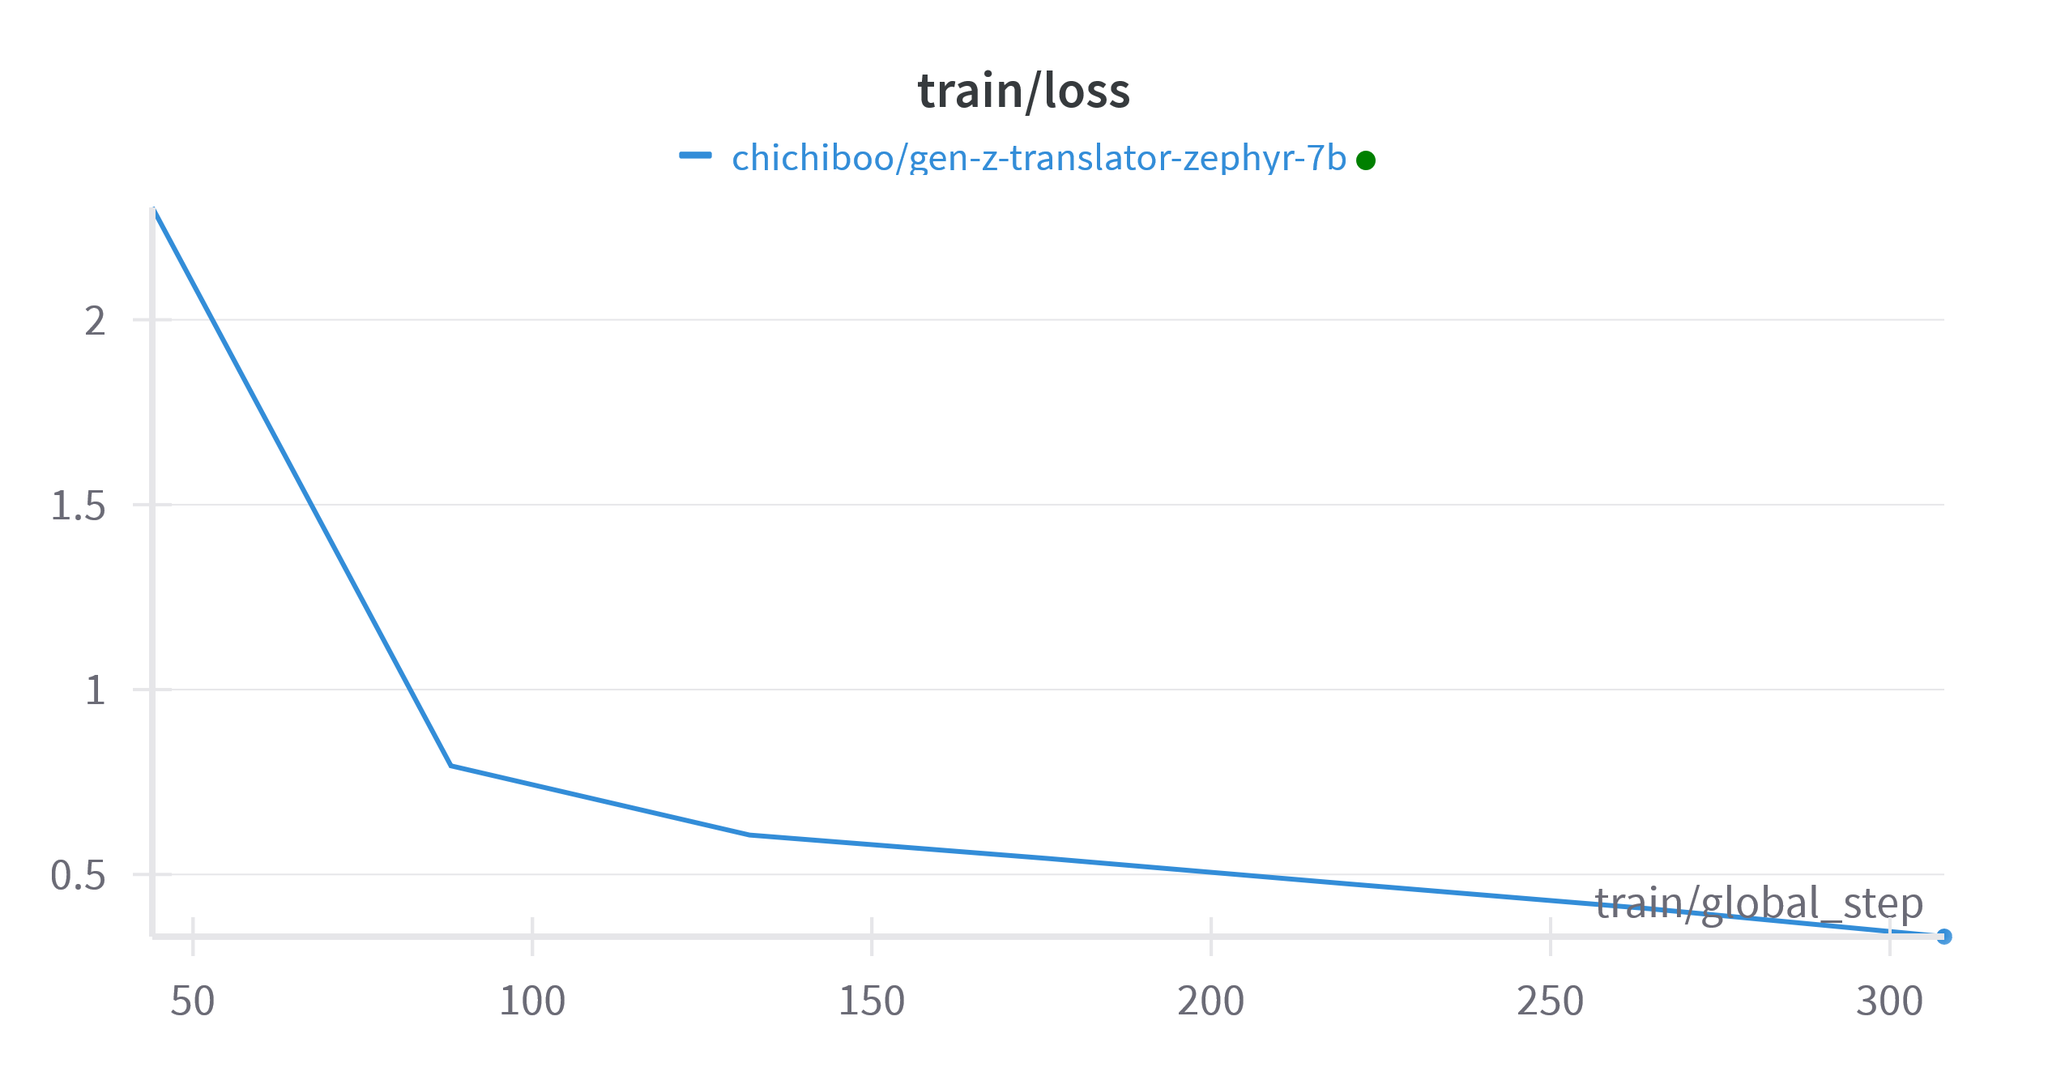
\includegraphics[scale=0.2]{figures/TrainLoss.png}
	\caption{Training loss curve of the fine-tuned model across training steps}
	\label{fig:train_loss}
\end{figure}
\begin{figure}[!htbp]
	\centering
	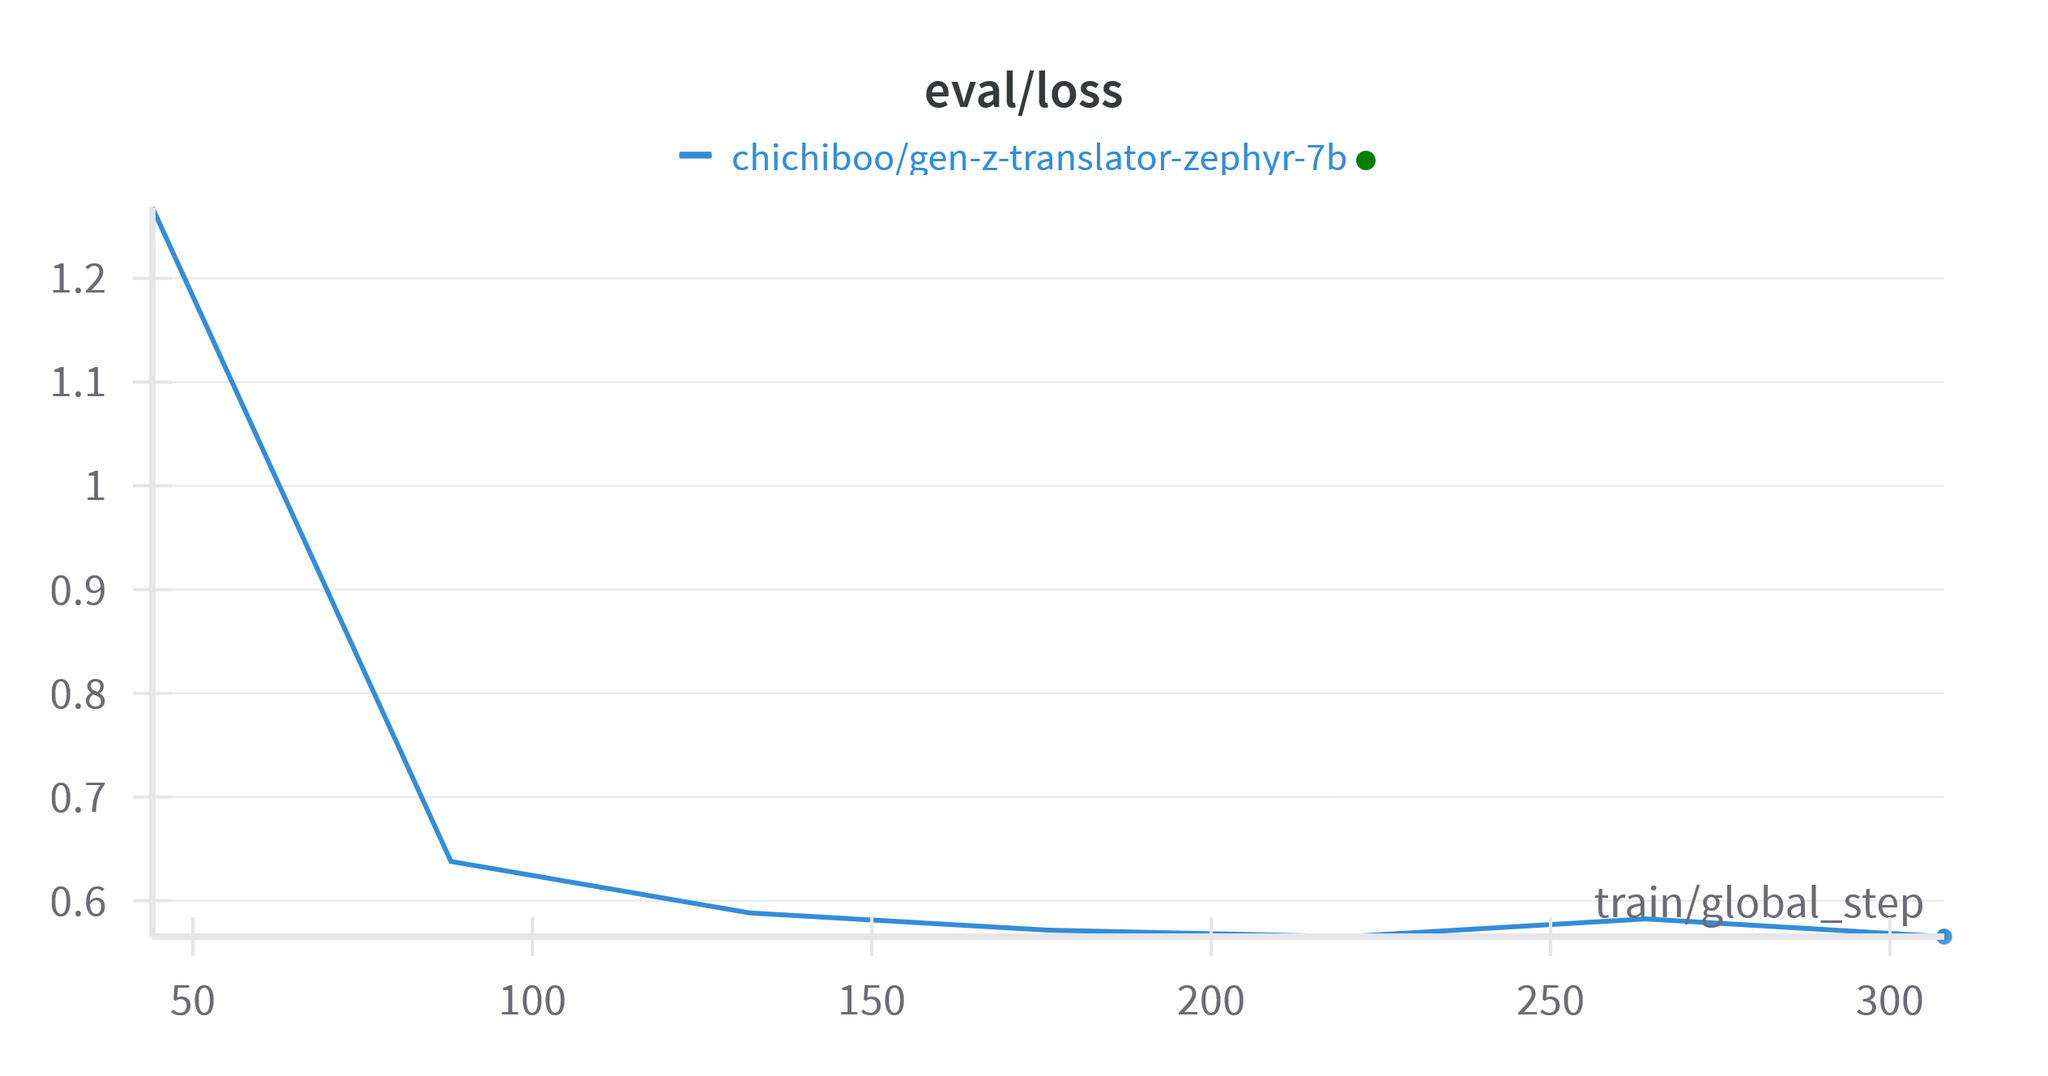
\includegraphics[scale=0.2]{figures/EvaluationLoss.png}
	\caption{Evaluation loss curve of the fine-tuned model across training steps}
	\label{fig:eval_loss}
\end{figure}
\begin{figure}[!htbp]
	\centering
	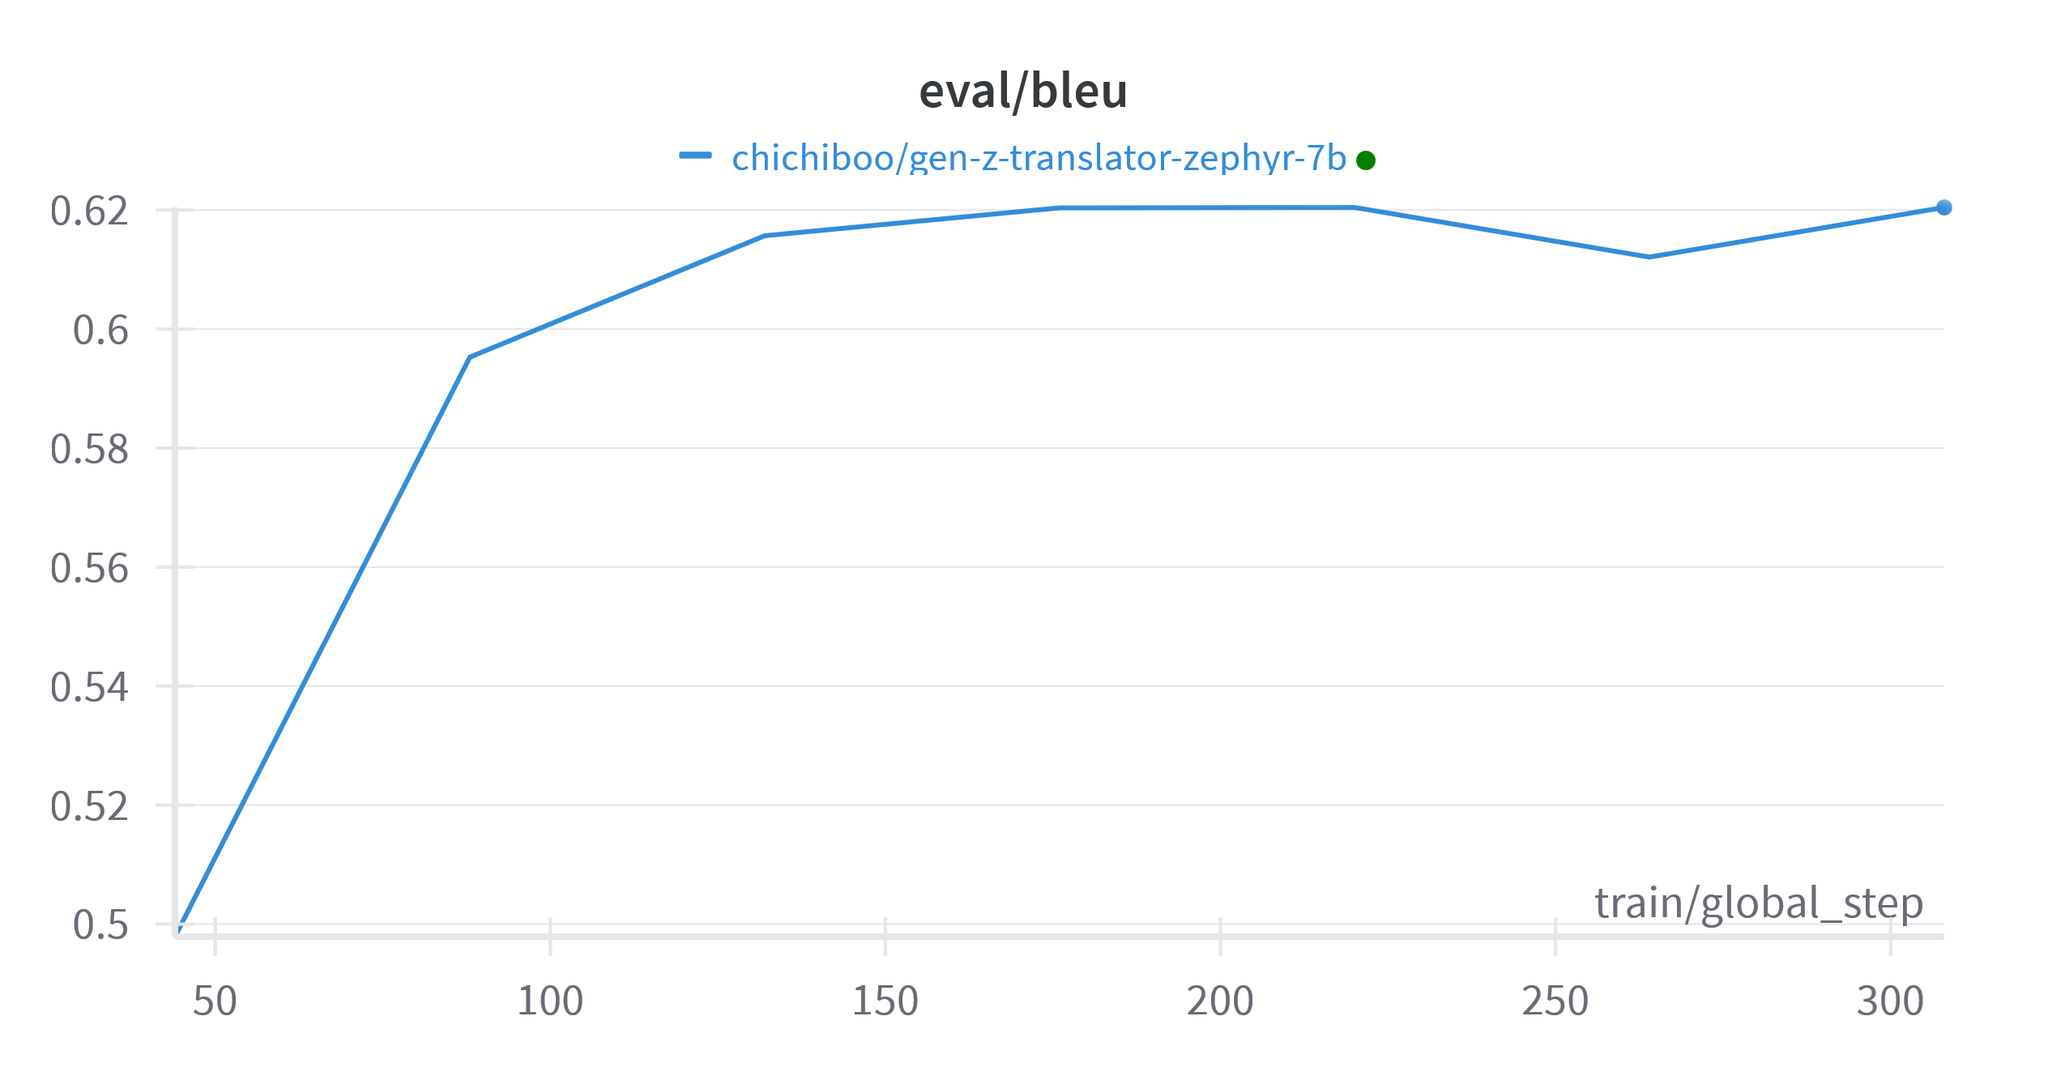
\includegraphics[scale=0.2]{figures/BLEUEvaluation.png}
	\caption{Evaluated using BLEU metric}
	\label{fig:bleu_eval}
\end{figure}
\begin{figure}[!htbp]
	\centering
	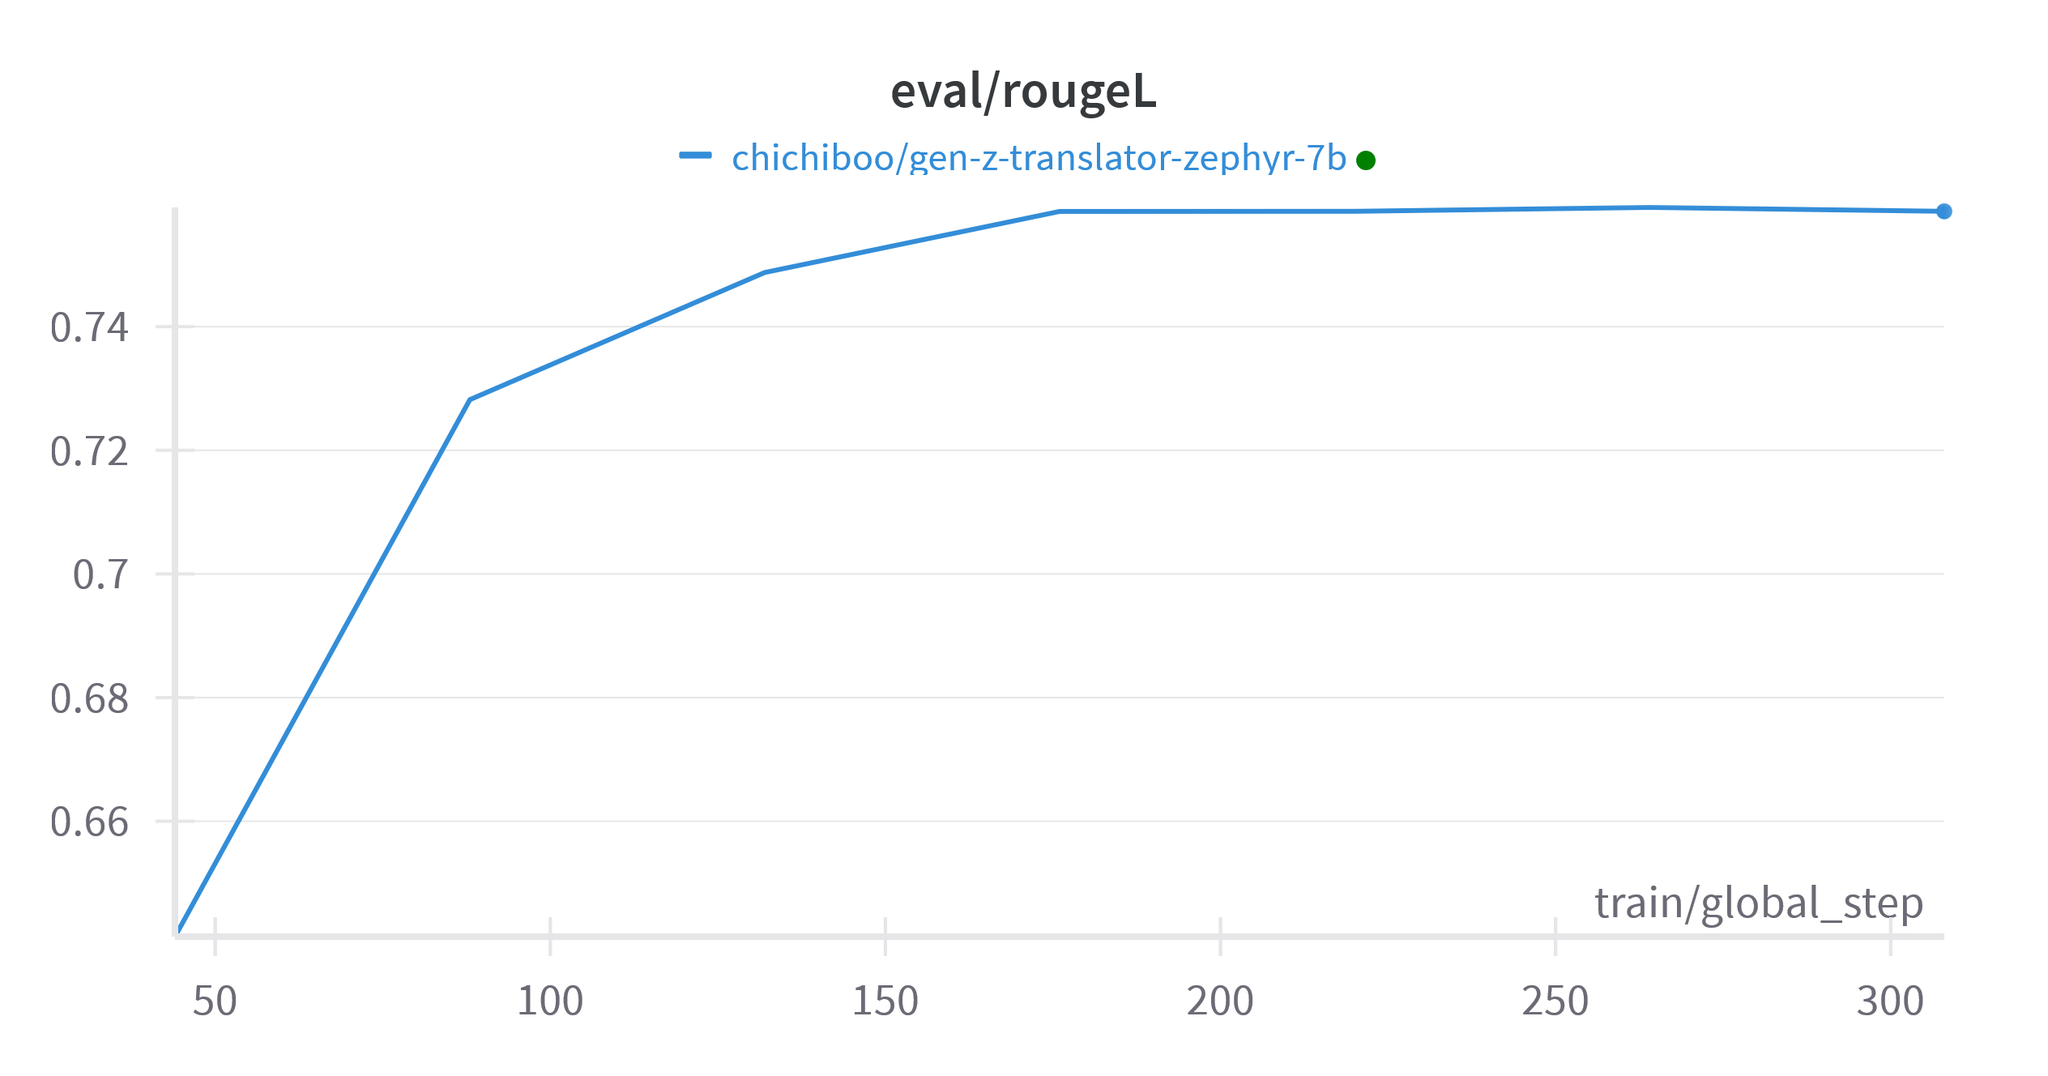
\includegraphics[scale=0.2]{figures/ROUGELEvaluation.png}
	\caption{Evaluated using ROUGE-L metric}
	\label{fig:rouge_eval}
\end{figure}
\FloatBarrier
\subsection{Text Generation}
A total of 170 sentences were translated using both the base zephyr-7b-beta model and the finetuned model. The translations are then filtered to remove duplicate answers between models or has minor differences such as punctuation or filler words that does not contribute to the meaning of the sentence. A total of 143 sentences then served as the dataset used to evaluate the performance of the model and comparing it with the other base model.

\subsection{Automatic Evaluation Metrics}
The dataset was automatically evaluated using BLEU and ROUGE metrics, specifically the ROUGE-L metric as the dataset do not contain newlines that ROUGE-Lsum uses to separate the input with. These scores were then averaged to determine the score of the models. The base model obtained a BLEU score of 0.8099 and ROUGE-L Score of 0.8336 and the fine-tuned model obtained a BLEU score of 0.8151 and ROUGE-L Score of 0.8396. While the difference between the models is minimal, this does not completely represent the performance of the models as these metrics are only used to determine if the generated text is close to the reference text, regardless of the context and the overall quality of the generated text. However, it does show that the fine-tuned model has little improvement over the base model.

\subsection{Manual Evaluation Metrics}
A manual evaluation was conducted by the researchers through a survey administered via Google Forms to determine which of the two models is preferred by Generation Z students at University of the Philippines Visayas (UPV). The survey comprised a total of 144 questions, which were distributed across five separate forms. The first form contained 20 questions, the second 19, the third 20, the fourth 20, the fifth 14, \textbf{and the sixth 50 amounting to 143 questions} in total. Each question presented two translation options: one generated by the fine-tuned model and the other by the base model. Respondents were asked to select the translation they preferred in each case.\textbf{ A total of 114 individuals participated in the survey, with 29, 22, 22, 21, and 20 respondents completing Forms 1 through 5, respectively. }

The data presented below illustrate respondent preferences between the base and fine-tuned models across the six survey forms, as well as the overall summary of the results. Each graph visualizes the outcomes for an individual form, specifically indicating both the raw number of responses and the corresponding percentages favoring each model. A systematic evaluation for each graph is provided as follows:

\begin{figure}[htbp]
	\centering
	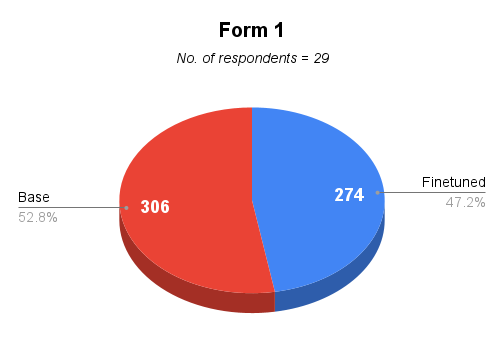
\includegraphics[scale=0.7]{figures/Form1.png}
	\caption{Form 1 Evaluation}
	\label{fig:form1}
\end{figure}

Figure \ref{fig:form1} shows that among the 29 respondents, 306 responses or 52.8 percent preferred the base model, while 274 responses or 47.2 percent favored the fine-tuned model. This indicates a slight preference for the base model in this particular form. Notably, this result deviates from the overall trend observed in the other four forms, where the fine-tuned model tends to be favored. Form 1 is the only instance in which the base model outperformed the fine-tuned model, suggesting that specific characteristics of this form may have influenced the preferences of the respondents. 


\begin{figure}[htbp]
	\centering
	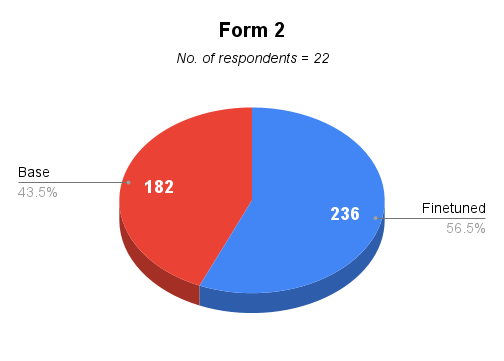
\includegraphics[scale=0.7]{figures/Form2.png}
	\caption{Form 2 Evaluation}
	\label{fig:form2}
\end{figure}

Figure \ref{fig:form2} implies that among 22 respondents, 236 responses, or 56.5 percent, favored the fine-tuned model, while 182 responses, or 43.5 percent, preferred the base model. This 13 percent margin reflects the clear preference for the fine-tuned model, which is consistent with the overall trend observed across the other forms. 

\begin{figure}[htbp]
	\centering
	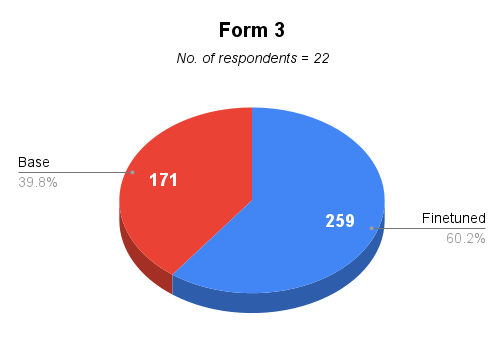
\includegraphics[scale=0.7]{figures/Form3.png}
	\caption{Form 3 Evaluation}
	\label{fig:form3}
\end{figure}

Figure \ref{fig:form3} illustrates that among the 22 respondents, the fine-tuned model received a significantly higher preference, with 259 responses or 60.2 percent, compared to the base model with 171 responses or 29.8 percent. This 20.4 percent margin represents the widest gap among all forms. This strongly indicates the superior performance of the fine-tuned model on translating, presented in Form 3. 

\begin{figure}[htbp]
	\centering
	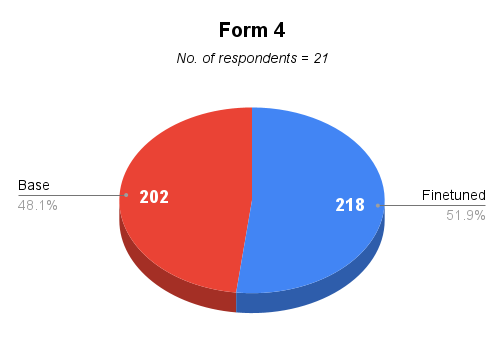
\includegraphics[scale=0.7]{figures/Form4.png}
	\caption{Form 4 Evaluation}
	\label{fig:form4}
\end{figure}

Figure \ref{fig:form4} highlights that the 21 respondents in Form 4 yielded a nearly even distribution of preferences, with 218 responses or 51.9 percent favoring the fined-tuned model and 202 responses or 48.1 percent preferring the base model. This narrow 3.8 percent difference suggests a comparable level of performance between the two models in this particular form. 

\begin{figure}[htbp]
	\centering
	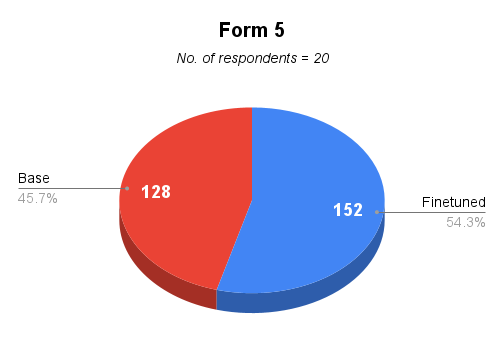
\includegraphics[scale=0.7]{figures/Form5.png}
	\caption{Form 5 Evaluation}
	\label{fig:form5}	
\end{figure}

Figure \ref{fig:form5} conveys that among the 20 respondents in Form 5, 152 responses or 54.3 percent selected the fine-tuned model, while 128 responses or 45.7 percent chose the base model. This 8.6 percent margin reinforces the general trend toward the fine-tuned model across all forms.

\begin{figure}[htbp]
	\centering
	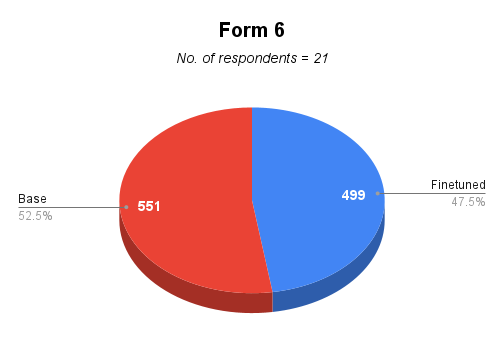
\includegraphics[scale=0.7]{figures/Form 6.png}
	\caption{Form 6 Evaluation}
	\label{fig:form6}	
\end{figure}

Figure \ref{fig:form6} indicates the results of the sixth form. 21 respondents in Form 6 showed a slight preference for the base model, garnering 52.5\%, over the fine-tuned model, with 47.5\%. Along with Form 1, this result contrasts with the overall trend observed across all gathered data.  

\begin{figure}[htbp]
	\centering
	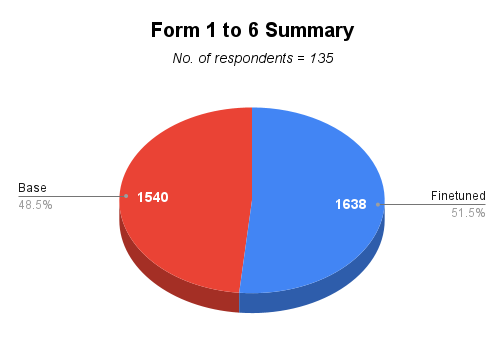
\includegraphics[scale=0.7]{figures/Summary.png}
	\caption{Summary Evaluation}
	\label{fig:summary}	
\end{figure}

Figure \ref{fig:summary} presents the overall summary across all five forms, with a total of 135 responsees garnered in the survey. In total, the fine-tuned model received 53.5\%, while the base model garnered 989 preferences or 46.5\%. The resulting 7\% margin between the two model indicates a moderate overall preference among Gen Z students at UPV for the fine-tuned model, suggesting its relatively better performance in meeting the participants' expectations for translation quality. 

\section{Summary}
The chapter presented the evaluation results and discussions on the performance of the fine-tuned language model for translating Gen Z internet slang into their formal translations. The dataset used for training consisted of 1,703 sentence pairs, combining original and publicly available data. The model was trained for seven epochs, with early stopping employed to prevent overfitting, which was evident from the divergence between training and validation losses.

Evaluation was conducted using both automatic and manual methods. The automatic evaluation, using BLEU and ROUGE-L metrics, showed marginal improvements in the fine-tuned model compared to the base model, suggesting slightly better alignment with reference translations. 

To support the results of automatic evaluation metrics, a manual evaluation was carried out through online surveys among Generation Z students at UPV. Participants compared translations from both models across six forms. Results showed a moderate overall preference for the fine-tuned model, with 53.5\% of responses in its favor. While one form showed a slight preference for the base model, the fine-tuned model was generally preferred, especially in Form 3 where it showed the largest margin.

In summary, the findings indicate that the fine-tuned model slightly outperformed the base model in terms of automatic metrics and showed a modest but consistent preference among target users, supporting its effectiveness in translating Gen Z slang into more formal language.